\documentclass[a4 paper]{article}
% Set target color model to RGB
\usepackage[inner=2.0cm,outer=2.0cm,top=2.5cm,bottom=2.5cm]{geometry}
\usepackage{setspace}
\usepackage{ulem}
%\usepackage[backend=biber,style=alphabetic,sorting=ynt]{biblatex}
\usepackage{natbib}
% \bibliographystyle{plainnat}
\bibliographystyle{unsrtnat}
%\usepackage[nottoc]{tocbibind}
% \addcontentsline{toc}{section}{References}
%\addbibresource{bib_Lab2.bib}
\usepackage{arydshln}
% \usepackage[rgb]{xcolor}
\usepackage[dvipsnames]{xcolor}
\colorlet{LightRubineRed}{RubineRed!70!}
\usepackage[most]{tcolorbox}
\usepackage{verbatim}
\usepackage{subcaption}
\usepackage{amsgen,amsmath,amstext,amsbsy,amsopn,tikz,amssymb,tkz-linknodes}
\usepackage{fancyhdr}
\usepackage[colorlinks=true, urlcolor=blue,  linkcolor=blue, citecolor=blue]{hyperref}
\usepackage[colorinlistoftodos]{todonotes}
\usepackage{rotating}
\usepackage{multicol}
\usepackage{graphicx}
%\usetikzlibrary{through,backgrounds}
\hypersetup{%
pdfauthor={Ashudeep Singh},%
pdftitle={Homework},%
pdfkeywords={Tikz,latex,bootstrap,uncertaintes},%
pdfcreator={PDFLaTeX},%
pdfproducer={PDFLaTeX},%
}
%\usetikzlibrary{shadows}
% \usepackage[francais]{babel}
\usepackage{booktabs}
\usepackage{amsmath}
\newcommand{\ra}[1]{\renewcommand{\arraystretch}{#1}}

\newtheorem{thm}{Theorem}[section]
\newtheorem{prop}[thm]{Proposition}
\newtheorem{lem}[thm]{Lemma}
\newtheorem{cor}[thm]{Corollary}
\newtheorem{defn}[thm]{Definition}
\newtheorem{rmk}[thm]{Remark}
\numberwithin{equation}{section}

\newcommand{\homework}[6]{
   \pagestyle{myheadings}
   \thispagestyle{plain}
   \newpage
   \setcounter{page}{1}
   \noindent
   \begin{center}
   \framebox{
      \vbox{\vspace{2mm}
    \hbox to 6.28in { {\bf IOC 5275:~Brain Computer Interface \hfill {\small (#2)}} }
       \vspace{6mm}
       \hbox to 6.28in { {\Large \hfill #1  \hfill} }
       \vspace{6mm}
       \hbox to 6.28in { {\it Instructor: {\rm #3} \hfill Group Number:  {\rm #5}} }% Student Id: {\rm #6}
       \hbox to 6.28in { {\it TA: #4  \hfill #6}}
      \vspace{2mm}}
   }
   \end{center}
   \markboth{#5 -- #1}{#5 -- #1}
   \vspace*{4mm}
}

\newcommand{\problem}[2]{~\\\fbox{\textbf{Problem #1}}\hfill (#2 points)\newline\newline}
\newcommand{\subproblem}[1]{~\newline\textbf{(#1)}}
\newcommand{\D}{\mathcal{D}}
\newcommand{\Hy}{\mathcal{H}}
\newcommand{\VS}{\textrm{VS}}
\newcommand{\solution}{~\newline\textbf{\textit{(Solution)}} }

\newcommand{\bbF}{\mathbb{F}}
\newcommand{\bbX}{\mathbb{X}}
\newcommand{\bI}{\mathbf{I}}
\newcommand{\bX}{\mathbf{X}}
\newcommand{\bY}{\mathbf{Y}}
\newcommand{\bepsilon}{\boldsymbol{\epsilon}}
\newcommand{\balpha}{\boldsymbol{\alpha}}
\newcommand{\bbeta}{\boldsymbol{\beta}}
\newcommand{\0}{\mathbf{0}}


\begin{document}
\homework{Lab2: EEG Preprocessing and Data Cleaning}{Due: 04/15/2021}{Chun-Shu Wei}{Min-Jiun Tsai}{2}{309554032, 309551176, 309540022, 0856642, 0716092, 0716085}
\noindent{\color{LightRubineRed} \rule{\linewidth}{1mm} }
\begin{center}
    \textbf{\Large{Submission Policy}}
\end{center}
\noindent{\color{LightRubineRed} \rule{\linewidth}{1mm} }
\par Read all the instructions below carefully before you start working on the assignment, and before you make a submission. For this assignment, please hand in the following your report (pdf) and code (.ipynb or .m file).
\begin{itemize}
    \item \textbf{PLAGIARISM IS STRICTLY PROHIBITED. (0 point for Plagiarism)}
    \item For mathematical problem(s), please show your work step by step and clarify statement of theorem you use (if any). Answering without mathematical derivations will get 0 point.
    \item Submission deadline: \textbf{2021.04.15 09:00:00 AM}. 
    \item \textbf{Late submission penalty formula:} $$original \ score\times(0.7)^{\#(days \ late)}$$ 
\end{itemize}
\noindent{\color{LightRubineRed} \rule{\linewidth}{0.1mm}}
\begin{center}
    \textbf{\large{File Format}}
\end{center}
\begin{itemize}
    \item Each group submits 1 report (.pdf and .tex file) and 1 code (.ipynb or .m).
    \item \textbf{Report} must contains observations, results and explanations. Please name your .pdf and .tex file as \textbf{5275\_Lab2\_GroupNum.pdf} and \textbf{5275\_Lab2\_GroupNum.tex},respectively.
    \item Paper submission is not allowed. \textbf{Please use our \LaTeX{} template to complete your report}.
    \item \textbf{Code} file must contains comments to explain your code. Please name your code file as\\ \textbf{5275\_Lab2\_GroupNum.ipynb/.m}
    \item Implementation will be graded by completeness, algorithm correctness, model description, and discussion.
    \item \textbf{Illegal format penalty:} $-5$ points for violating each rule of file format.
\end{itemize}
\noindent{\color{LightRubineRed} \rule{\linewidth}{0.1mm}}
\begin{center}
    \textbf{\large{Prerequest}}
\end{center}
To finish programming problem, you could choose Matlab or Python base on your programming preference.
\begin{multicols}{2}
\textbf{Matlab 2020a+}
\begin{itemize}
    \item \href{https://ca.nctu.edu.tw/installation/item/matlab-tah-standalone-ch}{NYCU installation page}
    \item \href{https://ca.nctu.edu.tw/manual/matlab/NCTU_MATLAB_TAH_stand_alone_installation_ch.pdf}{NCTU installation tutorial}
    \item \href{https://sccn.ucsd.edu/eeglab/downloadtoolbox.php}{EEGLab official installation page} (v2020.0+ is recommended)
\end{itemize}
\columnbreak
\textbf{Python 3.7+}
\begin{itemize}
    \item \href{https://mne.tools/stable/install/index.html}{MNE official installation page}  (0.20.7+ is recommended)
\end{itemize}
\end{multicols}
\noindent{\color{LightRubineRed} \rule{\linewidth}{0.1mm}}
\newpage
\section{Mathematical problem}
\subsection{Find the coefficients $b_n$ in Fourier sine series}
Let us begin with the Fourier sine series
\begin{equation}
    S(t)=\sum_{n=1}^\infty b_n\sin{\frac{n\pi t}{T}}, \ in \ the \ interval \ (0,T).
\end{equation}
To solve $b_n$ while $S(t)$ is given, we can use the key observation that $$\int_0^T \sin{\frac{n\pi t}{T}}\sin{\frac{m\pi t}{T}}dt=0 \ \forall m,n\in\mathbb{Z}, \  m\neq n$$ with $\sin{a}\sin{b}=\frac{1}{2}[\cos{(a-b)}-\cos{(a+b)}]$.
\begin{equation}
\begin{split}
\int_0^T \sin{\frac{n\pi t}{T}}\sin{\frac{m\pi t}{T}}dt&=\frac{1}{2}\int_0^T \cos{((n-m)\frac{\pi t}{T})}-\cos{((n+m)\frac{\pi t}{T})}dt\\&=\Big[\frac{T}{2\pi(n-m)}\sin{\frac{(n-m)\pi t}{T}}-\frac{T}{2\pi(n+m)}\sin{\frac{(n+m)\pi t}{T}}\Big|^T_{t=0}\Big]\\
&=0, \ \forall m,n\in\mathbb{N}, \ m\neq n
\end{split}
\end{equation} Let’s fix $m$, multiply $(1.1)$ by $\sin\frac{m\pi t}{T}$, and integrate the series $(1.1)$ term by term to get
\begin{equation}
\begin{split}
\int_0^T S(t)\sin{\frac{m\pi t}{T}}dt&=\int_0^T \Big(\sum_{n=1}^\infty b_n\sin{\frac{n\pi t}{T}}\Big)\sin{\frac{m\pi t}{T}}dt=\sum_{n=1}^\infty b_n\int_0^T \sin{\frac{n\pi t}{T}}\sin{\frac{m\pi t}{T}}dt=b_m\int_0^T \sin^2{\frac{m\pi t}{T}}dt
\end{split}
\end{equation} First, We can compute $\int_0^T\sin^2{\frac{m\pi t}{T}}dt$: \begin{equation}
\begin{split}
\int_0^T \sin^2{\frac{m\pi t}{T}}dt&=-\frac{T}{m\pi}\int_0^T\sin{\frac{m\pi t}{T}}d\cos{\frac{m\pi t}{T}}=-\frac{T}{m\pi}\Big[\sin{\frac{m\pi t}{T}}\cos{\frac{m\pi t}{T}}\Big|_{t=0}^T-\frac{m\pi}{T}\int_0^T \cos^2{\frac{m\pi t}{T}}dt\\&=-\frac{T}{m\pi}\Big[\sin{\frac{m\pi t}{T}}\cos{\frac{m\pi t}{T}}\Big|_{t=0}^T-\frac{m\pi}{T}\int_0^T 1-\sin^2{\frac{m\pi t}{T}}dt\Big]\\&=-\frac{T}{m\pi}\Big[\sin{\frac{m\pi t}{T}}\cos{\frac{m\pi t}{T}}\Big|_0^T\Big]+T-\int_0^T \sin^2{\frac{m\pi t}{T}}dt
\end{split}
\end{equation} $$\Rightarrow\int_0^T \sin^2{\frac{m\pi t}{T}}dt=\frac{1}{2}\Big\{-\frac{T}{m\pi}\Big[\sin{\frac{m\pi t}{T}}\cos{\frac{m\pi t}{T}}\Big|_0^T\Big]+T\Big\}=\frac{T}{2}\\\Rightarrow\int_0^T S(t)\sin{\frac{m\pi t}{T}}dt=b_m\int_0^T \sin^2{\frac{m\pi t}{T}}dt=b_m\frac{T}{2}$$
$$\Rightarrow b_m=\frac{2}{T}\int_0^T S(t)\sin{\frac{m\pi t}{T}}dt$$ This is the famous formula for the Fourier coefficients in the series $(1.1)$.
% Source Answer: https://stemjock.com/STEM%20Books/Strauss%20PDEs%202e/Chapter%205/Section%201/StraussPDEch5s1p05.pdf
\newline
\begin{tcolorbox}[colback=RubineRed!5!white,colframe=RubineRed!75!black]
\problem{1. Fourier Series}{10+5=15}
Suppose that the Fourier sine series of $g(x)=x \ on \ (0,l)$ is given by
\begin{equation}
    g(x)=\sum_{k=1}^{\infty} f_k(x)
\end{equation}
with conditions : $f_k:(0,l)\rightarrow\mathbb{R}$ is integrable and $\sum_{k=1}^\infty f_k(x)$ is uniformly convergent.
\subproblem{a} Find the \textbf{Fourier cosine series} of the function $\frac{x^2}{2}$ and the constant of integration (the $1^{st}$ term of cosine series).
\newline
\textcolor{red}{$a_0=\frac{2}{l}\int_0^l \frac{x^2}{2}dx=\frac{l^2}{3}$, $ a_n=\frac{2}{l}\int_0^l \frac{x^2}{2}\cos{\frac{n\pi x}{l}}dx=\frac{2l^2}{\pi^2n^2}\cos{n\pi}$}
\newline
\textcolor{red}{Fourier cosine series: $\frac{x^2}{2}=\frac{a_0}{2}+\sum_{n=1}^{\infty} {a_n\cos{\frac{n\pi x}{l}}} = \frac{l^2}{6}+2l^2\sum_{n=1}^{\infty}\frac{(-1)^n\cos(\frac{n\pi x}{l})}{(\pi n)^2}$}
\subproblem{b} Please exam whether the following series converges or not. Furthermore, find the sum of the series if it exists.
\begin{equation}
    \sum_{n=1}^\infty \frac{(-1)^{n+1}}{n^2}=?
\end{equation}
\newline
\textcolor{red}{Notice the result in (a): $\frac{x^2}{2}= \frac{l^2}{6}+2l^2\sum_{n=1}^{\infty}\frac{(-1)^n\cos(\frac{n\pi x}{l})}{(\pi n)^2}$}
\newline
\textcolor{red}{when $x=0$ $\Rightarrow 0= \frac{l^2}{6}+2l^2\sum_{n=1}^{\infty}\frac{(-1)^n}{\pi^2 n^2}\Rightarrow \frac{l^2}{6}=-2l^2\sum_{n=1}^{\infty}\frac{(-1)^n}{\pi^2 n^2}$}
\newline
\textcolor{red}{divide $\frac{2l^2}{\pi^2}$ in both side $\Rightarrow \frac{\pi^2}{12}=-\sum_{n=1}^{\infty}\frac{(-1)^n}{n^2}=\sum_{n=1}^{\infty}\frac{(-1)^{n+1}}{n^2}$}
\newline
\textcolor{red}{We get $\sum_{n=1}^{\infty}\frac{(-1)^{n+1}}{n^2}$ converges to $\frac{\pi^2}{12}$}
\end{tcolorbox}
\begin{tcolorbox}[colback=RoyalBlue!5!white,colframe=RoyalBlue!75!black]%neRed!75!black
\defn{Uniform Convergence}\\
Let $I$ be an interval on $\mathbb{R}$ and $f_k : I\rightarrow\mathbb{R}$ be a real-valued function on $I$. The sequence of functions $\{f_k\}_{k\in\mathbb{N}}$ is said to converge uniformly on $I$ to the function $f:I\rightarrow\mathbb{R}$ if $\forall\epsilon> 0,\exists N = N(\epsilon) \in\mathbb{N}$ such that $\forall x \in I$ and $k > N,|f_k(x)-f(x)| < \epsilon$.
\end{tcolorbox}
\subsection{Independent Component Analysis (ICA)}
\subsubsection{Motivation: Blind Source Separation (BSS)}
\par Blind Source Separation (BSS) is a method to estimate source signals from recorded signals which consist of mixed source signals and noise.
\begin{center}
    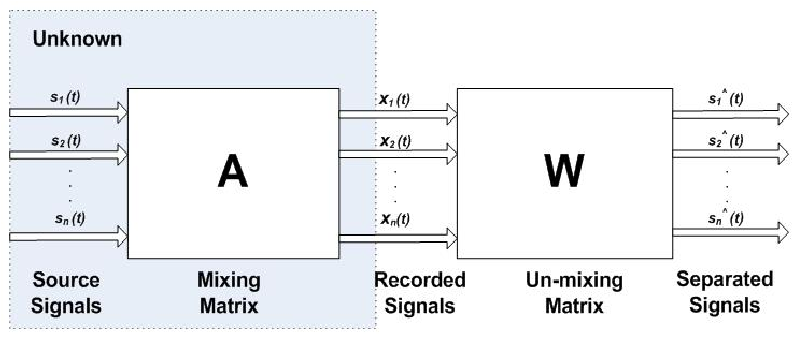
\includegraphics[height=4cm]{figure/Blind-source-separation-BSS-block-diagram-s-t-are-the-sources-x-t-are-the.png}\\
    \textbf{Figure: Blind Source Separation (BSS) [Naik and Kumar,2011]}
    %\label{fig:my_label}
\end{center}

\begin{tcolorbox}[colback=RoyalBlue!5!white,colframe=RoyalBlue!75!black,title=Model Formalization]
\par Let $n$ denotes number of source signal, $m$ denotes number of channel, and $d$ denotes dimension of signal. The matrix $S\in\mathbb{R}^{n\times d}$ denotes source signals. We assume that recorded signals $X=AS+E\in\mathbb{R}^{m\times d}$ are given by linear mixing system where $A\in\mathbb{R}^{m\times n}$ is the unknown mixing matrix and $E\in\mathbb{R}^{m\times d}$ denotes the noise. Basically, $m\geq n$
\end{tcolorbox}
The goal of BSS is to estimate $A$ and $S$ so that $\hat{S}$ provides unknown source signals as possible.
    $$X=AS+E\leftarrow X=\hat{A}\hat{S}$$
Since $m\geq n$, there are a lot of combinations $(A,S)$ satisfy $X=AS+E$.
    We could apply different types of constraint to solve this system:
\begin{multicols}{2}
\begin{itemize}
    \item PCA: Orthogonal constraint
    \item SCA: Sparsity constraint
\end{itemize}
\columnbreak
\begin{itemize}
    \item NMF: Non-negative constraint
    \item ICA: Statistically independent constraint
\end{itemize}
\end{multicols}
Therefore, there are many methods to solve the BSS problem depending on the constraints. What we used is depended on subject matter. In this lab, we only introduce \textbf{ICA}.
\subsubsection{Model of ICA}
\emph{The Cocktail Party Problem}
    \par Let $X$ be a recorded signal and $S$ is a source signal according to above formalization. We assume that $\{s_j\in\mathbb{R}^{d\times1}|j\in\mathbb{Z}_n\}$ is statistically independent.
\begin{equation}
X=\hat{A}\hat{S}\iff
\begin{bmatrix}
- & x_1^T & -\\
- & x_2^T & -\\
\vdots & \vdots & \vdots\\
- & x_{m}^T & -\\
\end{bmatrix}=
\hat{A}_{m\times n}
\begin{bmatrix}
- & \hat{s}_1^T & -\\
- & \hat{s}_2^T & -\\
\vdots & \vdots & \vdots\\
- & \hat{s}_{n}^T & -\\
\end{bmatrix}
\end{equation}
    %$$x_{ik}=\sum_{j=1}^n a_{ij}s_{jk}, \ \forall k\in\mathbb{Z}_d, \ \forall i\in\mathbb{Z}_{ch}$$
Independent Component Analysis is to estimate the independent component $S$ from $X$.
\begin{tcolorbox}[colback=RoyalBlue!5!white,colframe=RoyalBlue!75!black]
\textbf{Hypothesis of ICA}
\begin{itemize}
    \item $\{s_j\in\mathbb{R}^{d\times1}|j\in\mathbb{Z}_n\}$ statistically independent, that is, $P(s_1,...,s_n)=\prod_{j=1}^n P(s_j)$
    \item $\{s_j\in\mathbb{R}^{d\times1}|j\in\mathbb{Z}_n\}$ follows the Non-Gaussian distribution.
    \item $A$ is regular
\end{itemize}
Therefore, we could rewrite the model as $\hat{S}=\hat{B}X$ where $\hat{B}=\hat{A}^{-1}$. It's only necessary to estimate $B$ (compute $\hat{B}$) so that $\{s_j\in\mathbb{R}^{d\times1}|j\in\mathbb{Z}_n\}$ is independent.
\tcblower
\defn{White signal}\\
White signals are defined as any $z\in\mathbb{R}^{d\times1}$ which satisfying 
\begin{itemize}
    \item Zero mean: $E[z]=\textbf{0}=m_z$
    \item Unit covariance: $C_z=E[(z-m_{z})(z-m_{z})^T]=E[zz^{T}]=I_d$
\end{itemize}
\end{tcolorbox}
\textbf{Note}: If $m_z=\textbf{0}$, then the correlation matrix $R_z=C_z+m_zm_z^T=C_z$.
Recall that recorded signals are $X=\hat{A}\hat{S}$. ICA solve $\hat{S}$ by $\hat{S}=\hat{B}X$.
\begin{tcolorbox}[colback=RubineRed!5!white,colframe=RubineRed!75!black]
\problem{2: Whiteness property is preserved under orthogonal transformations}{5}
Assume that an orthogonal transformation $U\in\mathbb{R}^{d\times d}$ and $z$ is white, please prove that
\begin{equation}
    m_{Uz}=m_z \ \& \ C_{Uz}=C_z
\end{equation}
\newline
\textcolor{red}{We know $U$ is an orthogonal matrix\newline
So we can get $(Uz)^T(Uz)=z^TU^TUz=z^TIz=z^Tz$ \newline
1. Prove $m_{Uz}=m_z$:\newline
\hspace*{0.5cm} First we have $(Uz)^T(Uz)=z^Tz$\newline
\hspace*{0.5cm} $\rightarrow(Uz-m_{Uz})^T(Uz-m_{Uz})=(z-m_z)^T(z-m_z)$ \newline
\hspace*{0.5cm} $\rightarrow(Uz-m_{Uz})^T(Uz-m_{Uz})=z^Tz$\hspace*{0.5cm}$\because m_z=0$\newline
\hspace*{0.5cm} $\rightarrow m_{Uz}=0=m_z$\newline
2. Prove $C_{Uz}=C_z=I_d$:\newline
\hspace*{0.5cm} $C_{Uz}=E[(Uz-m_{Uz})(Uz-m_{Uz})^T]$\newline
\hspace*{0.5cm} $m_{Uz}=0$ from previous provement $\rightarrow C_{Uz}=E[Uz(Uz)^T]=E[Uzz^TU^T]$ \newline
\hspace*{0.5cm} $\rightarrow C_{Uz}=E[UI_dU^T]=E[UU^TI_d]=E[II_d]$\newline
\hspace*{0.5cm} $\rightarrow C_{Uz}=E[I_d]=I_d=E[zz^T]=C_z$
}
\end{tcolorbox}
\textbf{From now on we assume that $m=n$} to simplify the model. Whitening is useful for PCA and simplifies ICA problem.
If we denote whitening signal as 
\begin{equation}
Z_{d\times m}=V_{d\times d}X^T_{d\times m}\iff
\begin{bmatrix}
| & | &  \hdots & | \\
z_1 & z_2 & \hdots & z_m \\
| & | & \hdots & | \\
\end{bmatrix}=V_{d\times d}
\begin{bmatrix}
| & | & \hdots & |\\
x_1 & x_2 & \hdots & x_m\\
| & | & \hdots & |\\
\end{bmatrix}
\end{equation}
where $V\in\mathbb{R}^{d\times d}$ is a whitening matrix of $X_{m\times d}$, then model becomes
\begin{equation}
    \hat{S}^T_{d\times m}=U_{d\times d}Z_{d\times m}=U_{d\times d}V_{d\times d}X^T_{d\times m}=\hat{B}_{d\times d}X^T_{d\times m}\iff\begin{bmatrix}
| & | &  \hdots & | \\
\hat{s}_1 & \hat{s}_2 & \hdots & \hat{s}_m \\
| & | & \hdots & | \\
\end{bmatrix}=\hat{B}_{d\times d}
\begin{bmatrix}
| & | & \hdots & |\\
x_1 & x_2 & \hdots & x_m\\
| & | & \hdots & |\\
\end{bmatrix}% =Z_{d\times n}=U_{d\times d}V_{m\times n}X_{m\times d}=BX
\end{equation}
where $U\in\mathbb{R}^{d\times d}$ is an orthogonal transformation matrix.\\ \textbf{Hence it's necessary to estimate $U$!}

\par The gaussianity of $X$ (sums of non-gaussian random variables) must be larger than $S$ (original) according to Central Limit Theorem.
Let $\{x_j\in\mathbb{R}^{d\times1}|j\in\mathbb{Z}_m\}$ be the observed signals, we want to maximize the non-gaussianity of source signals $s_j=Bx_j$.\\
\begin{center}
    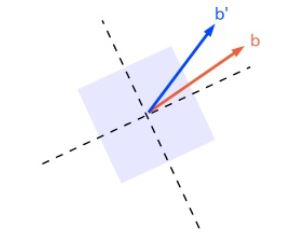
\includegraphics[height=4cm]{figure/nongaussianity.JPG}
    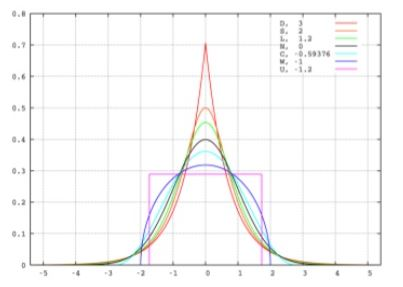
\includegraphics[height=4cm]{figure/distribution.JPG}\\
    \textbf{Figure:  (Left) The Non-gaussianity of $b$ is larger than $b^{'}$, (Right) Distributions [Yokota, 2012]}
\end{center}
\begin{tcolorbox}[colback=RoyalBlue!5!white,colframe=RoyalBlue!75!black,title=Kurtosis is a measure of non-gaussianity]
    \defn{Kurtosis}\\
        for a random variable $y\in\mathbb{R}^{d\times 1}$,
       $$kurt(y)=E[y^4]-3(E[y^2])^2$$
    \tcblower
    That is, for white signal $z\in\mathbb{R}^{d\times1}$, $$kurt(z)=E[z^4]-3(E[z^2])^2=E[z^4]-3$$
    Which means we could solve ICA problem by
    \begin{equation}
        \hat{b}=\max_{b}\large\|kurt(b^Tx)\large\|
    \end{equation}
\end{tcolorbox}
We consider $z=Vx$ is a white signal given from source signal $x$, then we could rewrite (1.11) as: 
\begin{tcolorbox}[colback=RubineRed!5!white,colframe=RubineRed!75!black]
\problem{3: Solving ICA problem by kurtosis}{10}
\begin{equation}
    \max \large\|kurt(w^Tz)\large\| \ with \ w^Tw=1
\end{equation}
% Comment: In the objective, we wrote ``Practice writing proofs'' but this is rather simple and not very rigorous?
\textcolor{red}{\newline First we rewrite the kurt func: $kurt(y)=E[y^4]-3(E[y^2])^2=E[(y^Ty)^2]-3(E[y^Ty])^2$\newline
Def $J(W)=kurt(w^Tz), F(w)=||J(W)||$, goal is to find $max(F(w))$ with $w^Tw=1$\newline
Solution: $J(w)=kurt(w^Tz)=E[(w^Tz)^4]-3E[(w^Tz)^2]^2$\newline
\hspace*{0.5cm} Def. $y=w^Tz$, then $y^Ty=z^Tww^Tz$ def= $h(w)$\newline
\hspace*{1cm} $\rightarrow h'(w)=2zz^Tw$\newline
\hspace*{0.5cm} $J(w)=kurt(y)=E[(y^Ty)^2]-3(E[y^Ty])^2=E[h(w)^2]-3E[h(w)]^2$\newline
\hspace*{1cm} $\rightarrow J'(w)=2E[h(w)h'(w)]-6E[h(w)]E[h'(w)]$\newline
\hspace*{1cm} $\rightarrow J'(w)=2\times 2E[(z^Tww^Tz)(zz^Tw)]-6\times 2E[z^Tww^Tz]E[zz^Tw]$\newline
\hspace*{1cm} $\rightarrow J'(w)=4(E[(z^Tww^Tz)(zz^Tw)]-3E[z^Tww^Tz]E[zz^Tw])$\newline
\hspace*{0.5cm} then we can get $F'(w)=\frac{\partial||J||}{\partial w}=4sgn(kurt(w^Tz))(E[(z^Tww^Tz)(zz^Tw)]-3E[z^Tww^Tz]E[zz^Tw])$\newline
\hspace*{0.5cm} then we just need to find $w$ that can make $F'(w)=0$ to get the $max||kurt(w^Tz)||$
}
\end{tcolorbox}
% \newpage
\section{Multiple choices}
Please give a brief explanation for option(s) you choose. Answering without any description will get 0 point.
\begin{tcolorbox}[colback=RubineRed!5!white,colframe=RubineRed!75!black]
\problem{4}{5}
The image here shows a \textbf{2-second} period of EEG from several different electrodes. What is the nature of the oscillating signal shown in the green box? \textbf{Select all correct options.}
\begin{multicols*}{2}
\begin{center}
    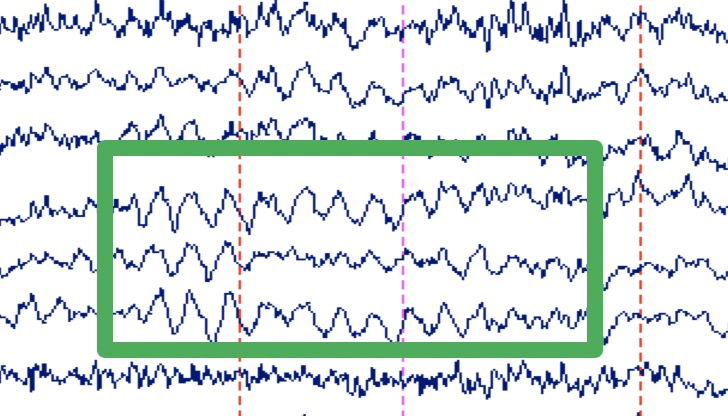
\includegraphics[height=4cm]{figure/Alpha.png}
    %\caption{Caption}
    %\label{fig:my_label}
\end{center}
\columnbreak
\begin{itemize}
    \item[(A)]It is a 1 Hz oscillation
    \item[(B)]It is a 5 Hz oscillation
    \item[(C)]It is a 10 Hz oscillation
    \item[(D)]It is a delta-band oscillation
    \item[(E)]It is a theta-band oscillation
    \item[(F)]It is an alpha-band oscillation
\end{itemize}
\end{multicols*}
\textcolor{red}{Answer: (C), (F)\newline Explanation: We def k waves in one second as k Hz. In this EEG diagram, we can do a simply counting. In each row, there has more than 20 peaks. Hence, (A) and (B) are impossible, (C) can be one of answer. Following the def. of $\theta$, $\delta$, $\alpha$-wave, $\delta$-wave is under 4Hz, $\theta$-wave is ranged in 4-8Hz, $\alpha$-wave is ranged in 8-13Hz. Hence, answer should be (F). }
\end{tcolorbox}
\begin{tcolorbox}[colback=RubineRed!5!white,colframe=RubineRed!75!black]
\problem{5}{5}
Which of the following statements are true of the frequency response function shown below? 
\begin{multicols*}{2}
\begin{center}
    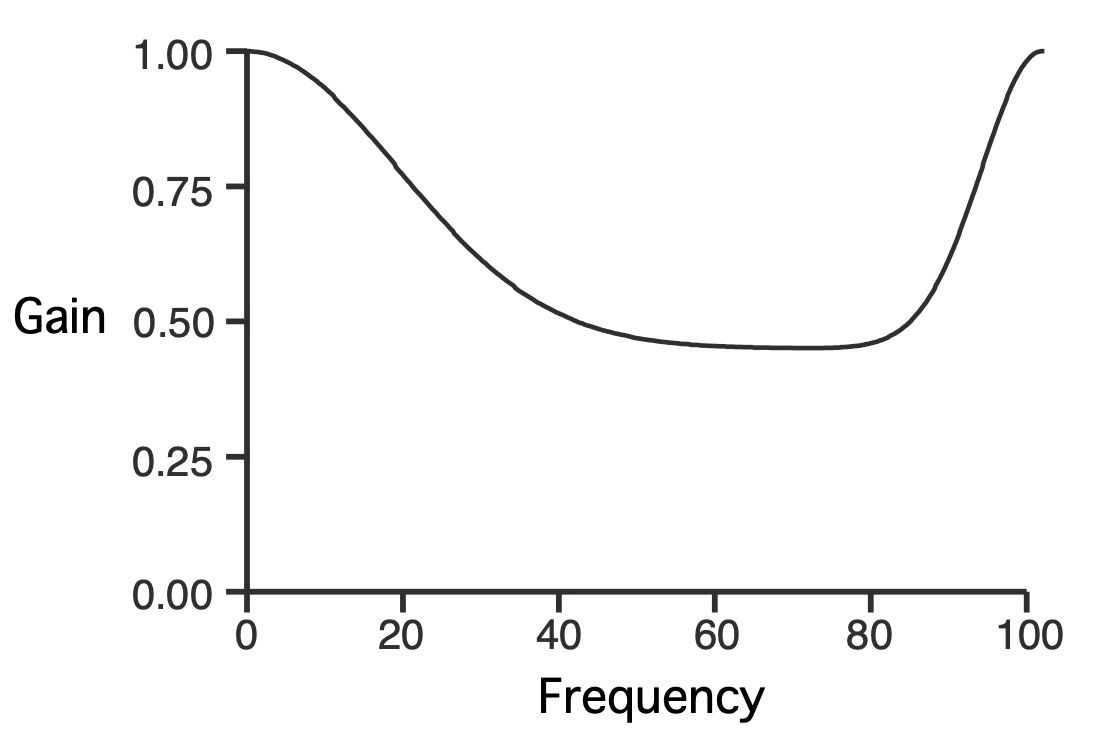
\includegraphics[height=5cm]{figure/Frequency-Response.png}
\end{center}
\columnbreak
\begin{itemize}
    \item[(A)] This filter would almost completely eliminate very low frequencies (because the gain is near 1.00 for low frequencies).
    \item[(B)]This filter would have very little effect on very low frequencies (because the gain is near 1.00 for low frequencies).
    \item[(C)]This filter would reduce frequencies of ~40-80 Hz by 50\% (because the gain is near 0.50 for these frequencies).
    \item[(D)] This is a high-pass filter.
    \item[(E)] This is a low-pass filter. 
\end{itemize}
\end{multicols*}
\textcolor{red}{Answer: (B), (C)\newline 
Explanation: The gain in big in low frequencies, so (A) is wrong. We can observe the phenomenon described in (B), (C) in the diagram. (D), (E) are wrong because it is a band-stop filter.}
\end{tcolorbox}
\section{Programming problem}
Please use the data: sXD\_5678.set to answer the following problems.
\subsubsection{Dataset Information}
The solid black arrows represent driving trajectory. The empty  circle represents deviation onset. The double circle represents response onset. The circle with a cross represents end of response. 
% An event-related lane-departure driving task was used to assess objectively and quantitatively fluctuations in driving (behavioral) performance over long periods. Each driving session lasted 40–60 min, 
which was sufficient for subjects to experience fatigue.
\begin{center}
    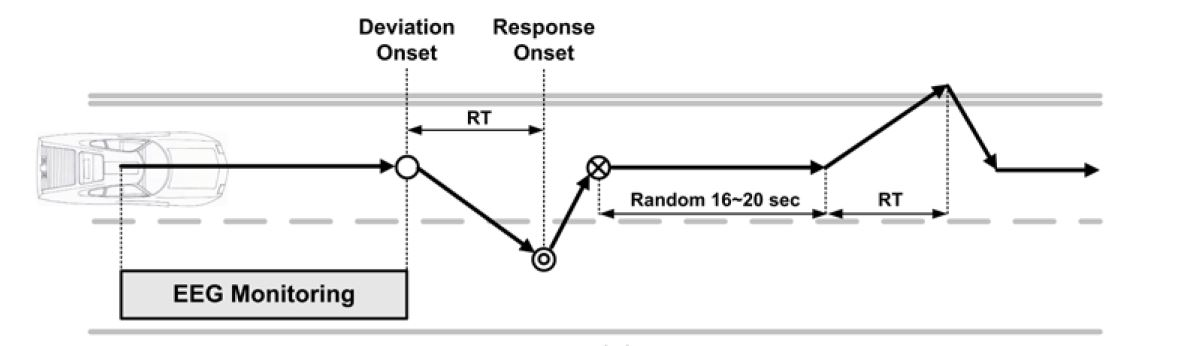
\includegraphics[height=3cm]{figure/lane_keeping.JPG}\\
    \textbf{Figure: Event-related lane-departure task}\\
    \textbf{[Kuan-Chih Huang and Jung,2016],[Chin-Teng Lin and Jung, 2010]}
\end{center}
\begin{tcolorbox}[colback=RubineRed!5!white,colframe=RubineRed!75!black]
\problem{6}{2+1+1+1+4+1=10}
Please following the following steps:  
\begin{itemize}
    \item[1.] Plot 2D channel location map and re-reference data by $\frac{A1+A2}{2}$.
    \item[2.] Down-sampling to $250Hz$.
    \item[3.] Run ICA and record computational time of ICA by code.
    \item[4.] Plot component map in 2D.
    \item[5.] Indicate noise component(s) if it exist and explain reason why you identify this component as a noise or artifacts.
    \item[6.] Plot first 10-second channel data before and after deleting noise/artifact component(s). 
\end{itemize}
\textcolor{red}{(5) component which has a smaller ID is an important component, which can't be deleted as possible as we can, and we can identify which ICA component is noise by taking a look at the ICA component 2D graph, we mainly want to remove muscle, ocular artifacts and other noise. The ocular artifact has relatively strong power in the part of the eye. In component 2, which has a strong ocular artifact. And for ICA component 0, which is a muscle artifact. There are many other artifacts, like only one specific channel has a strong power ICA component, that is ICA component with noise, which can be deleted. ICA component 1, we think is caused by "vehicle position" channel, but it can't be removed, because this component is the main eeg signal.
}
\end{tcolorbox}
\begin{tcolorbox}[colback=RubineRed!5!white,colframe=RubineRed!75!black]
\problem{7}{0+0+0+1+1+4+1+8+5=20}
Delete vehicle position channel and then:  
\begin{itemize}
    \item[1.] Plot 2D channel location map and re-reference data by $\frac{A1+A2}{2}$.
    \item[2.] Down-sampling to $250Hz$.
    \item[3.] Bandpass filtering $[1,50]Hz$ 
    \item[4.] Run ICA and record computational time of ICA by code.
    \item[5.]Plot component map in 2D.
    \item[6.] Indicate noise component(s) if it exist and explain reason why you identify this component as a noise or artifacts.
    \item[7.] Plot first 10-second channel data before and after deleting noise/artifact component(s).
\end{itemize}
\textcolor{red}{(6)component which has a smaller ID is an important component, hich can’t be deleted as posible as we can, and we can identify which ICA component is noise by taking a look at the ICA component 2D graph. We mainly want to remove muscle, ocular artifacts and other noise. The ocular artifact has relatively strong power in the part of the eye. In component 1, which has a strong ocular artifact. And for ICA component 0, which is a muscle artifact. There are many other artifacts, like only one specific channel has a strong power ICA component, that is ICA component with noise,which can be deleted.\newline}
After above preprocessing steps... ...
\subproblem{a} Compare results (e.g. component map) and try to explain your observations.
\newline
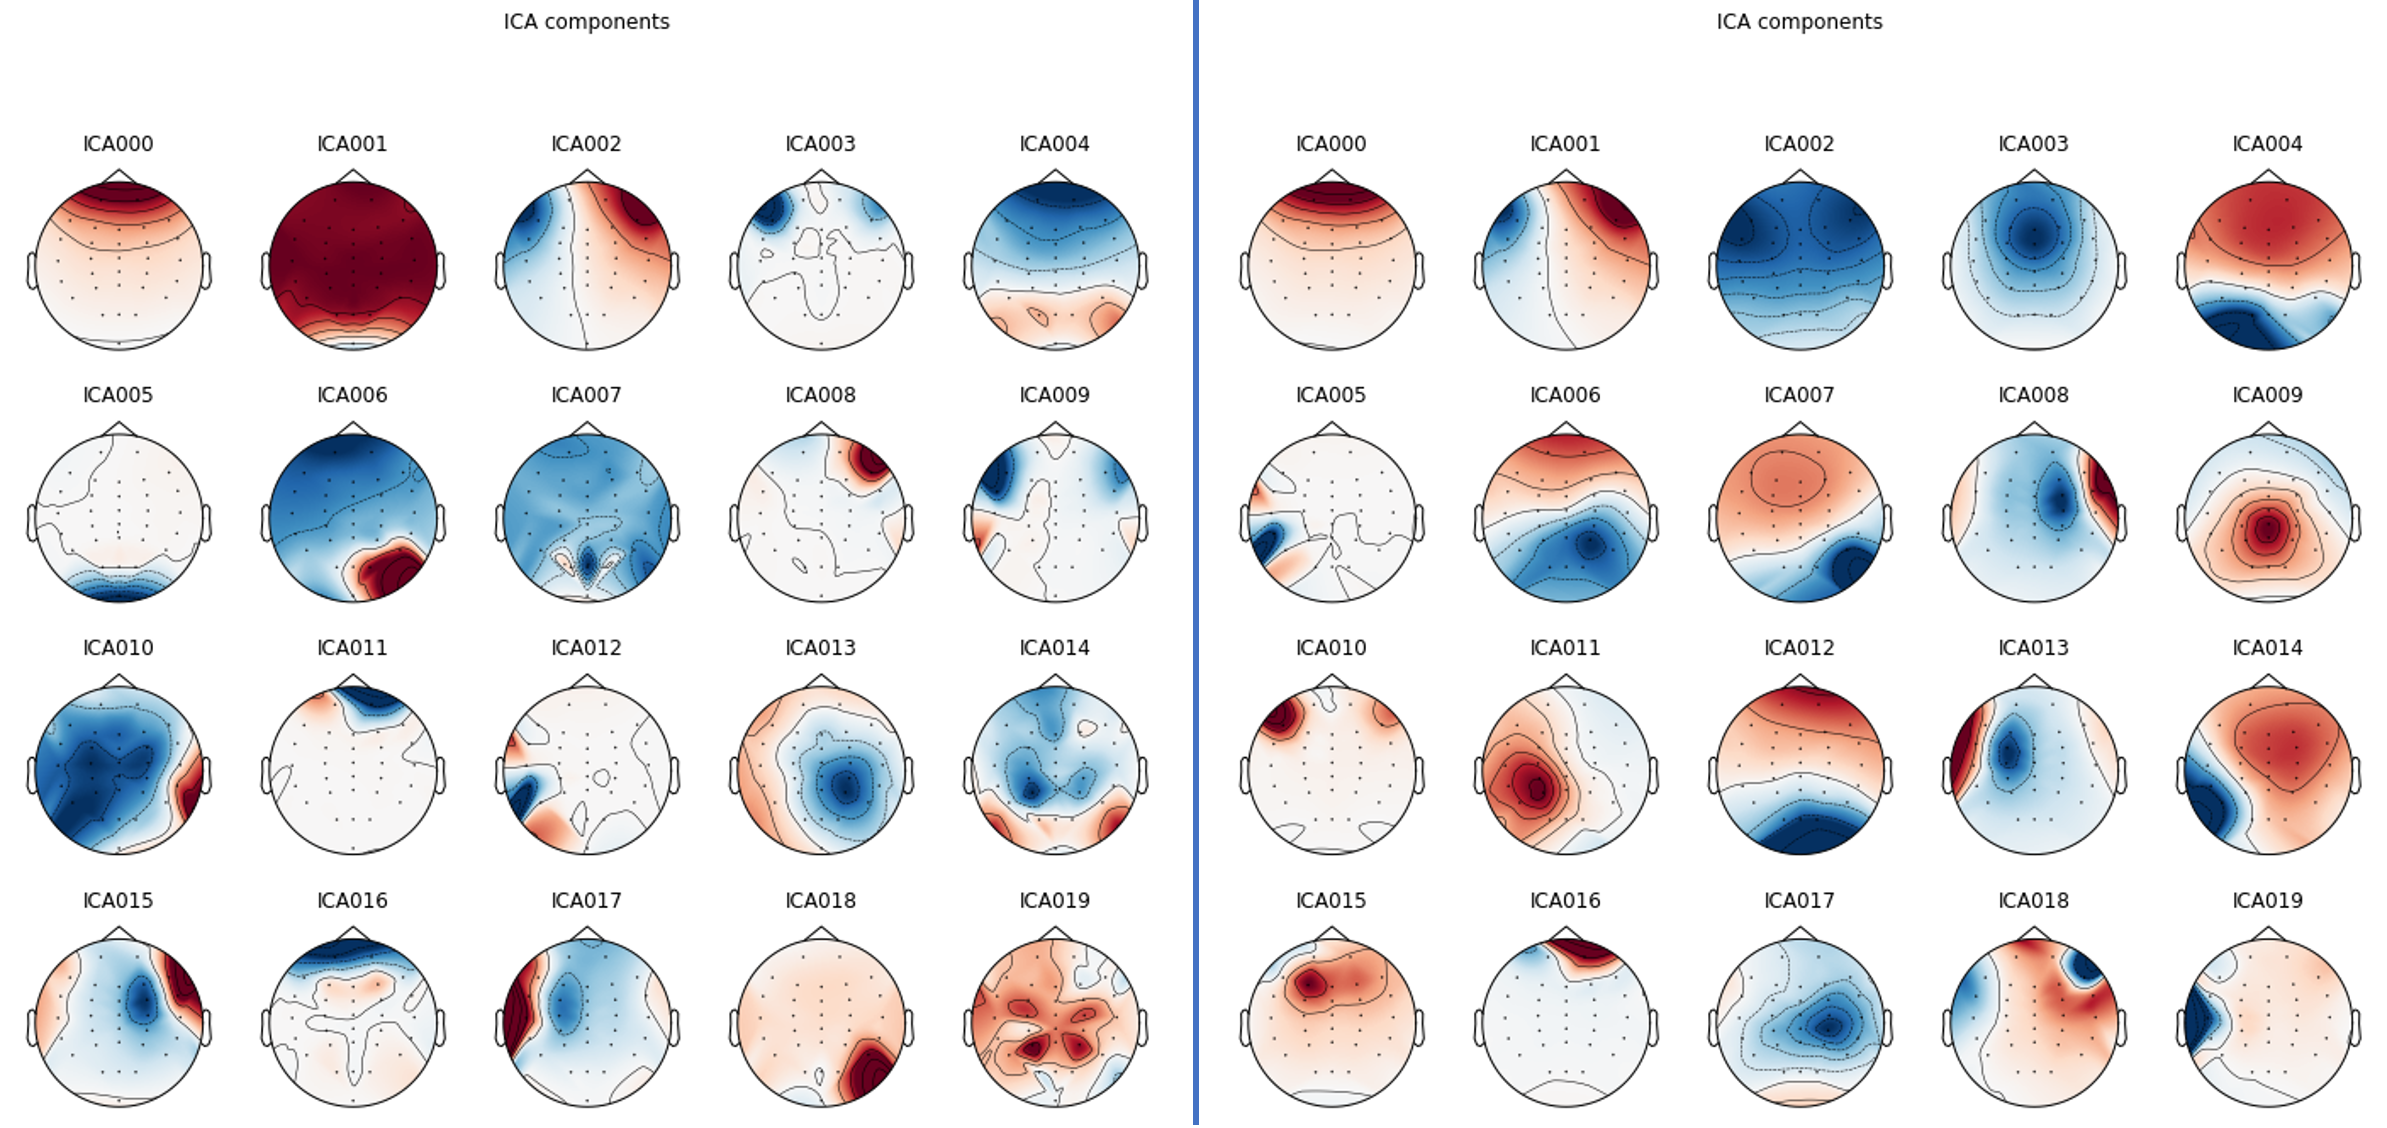
\includegraphics[height=4cm]{img/ica_res.png}\\
\textcolor{red}{[a.0] (problem 6 ICA component vs problem 7 ICA component)\newline there are two main difference between problem 7 and problem 8: 1. having "vehicle position" or not 2. having using bandpass filter(1~50 Hz) or not.\newline In problem 6, eeg signal(having "vehicle position" channel) will produce bad ICA components, because "vehicle position" is not eeg signal and it isn't related to eeg signal, so "vehicle position" in eeg signal should be removed.\newline Bandpass filter(1~50 Hz)can filter out lots of unnecessary noise (Because there has no value that is smaller than 1 Hz and larger than 50 Hzin brain wave). After doing ICA, you can further filter out more artifacts (such as ocular artifacts, muscle artifacts, etc.). But if you do ICA without using a bandpass filter. The power spectrum in eeg signals will be out of the range of 1-50 Hz after removing the ICA components. Which means eeg signals still have noise after removing the ICA components.}
\subproblem{b} Explain why it takes less time this time?
\textcolor{red}{\newline ICA algorithm is mainly run in a loop, and it stops when the best component is separated. In problem 7, eeg signals don’t have vehicle position, which is not related to eeg signal. removing the "vehicle position" channel makes it easier to find ICA components in eeg signals.\newline In contrast, an eeg signal that contains a "vehicle position" channel that makes it hard to find the best ICA component, just because "vehicle position" is not related to eeg. So when eeg runs with the ICA algorithm, it runs more loops to find the best component, that takes a lot of time.}
\end{tcolorbox}

\begin{tcolorbox}[colback=RubineRed!5!white,colframe=RubineRed!75!black]
\problem{8}{10+10+10=30}
Design your own EEG preprocessing strategy:
\subproblem{a} Describe your design idea (e.g. Apply CleanLine function in EEGLab to eliminate environmental artifacts and apply lowpass filtering to remove drift... ...)
\textcolor{red}{\newline Step 1. Set Reference by average: We avoided using 'A1' and 'A2' as our reference, instead, we set the average of our data as reference after we've done the previous steps to make sure our data is as clean as possible.
\newline Step 2. Bandpass filter [1, 50] Hz to remove environmental noise
\newline Step 3. Down Sampling to 250 Hz to save computational time
\newline Step 4. Drop the channel 'vehicle positio','A1' and 'A2', we dropped channel 'vehicle positio' since it wasn’t the signal source we're interested in, also, 'A1' and 'A2' were be the reference in our preprocessing strategy, instead, we used the average of the signal as our reference.
\newline Step 5. Run ICA and Remove bad components: We put our data into the ICA algorithm, but instead of indicating bad components manually, we used an experimental function "detect\_artifacts() provided by the MNE, due to our lack of experience in identifying corrupted components, hoping it would brought us better result.
}
\subproblem{b} Compare the performance (computational time) and results with Problem 7.
\newline
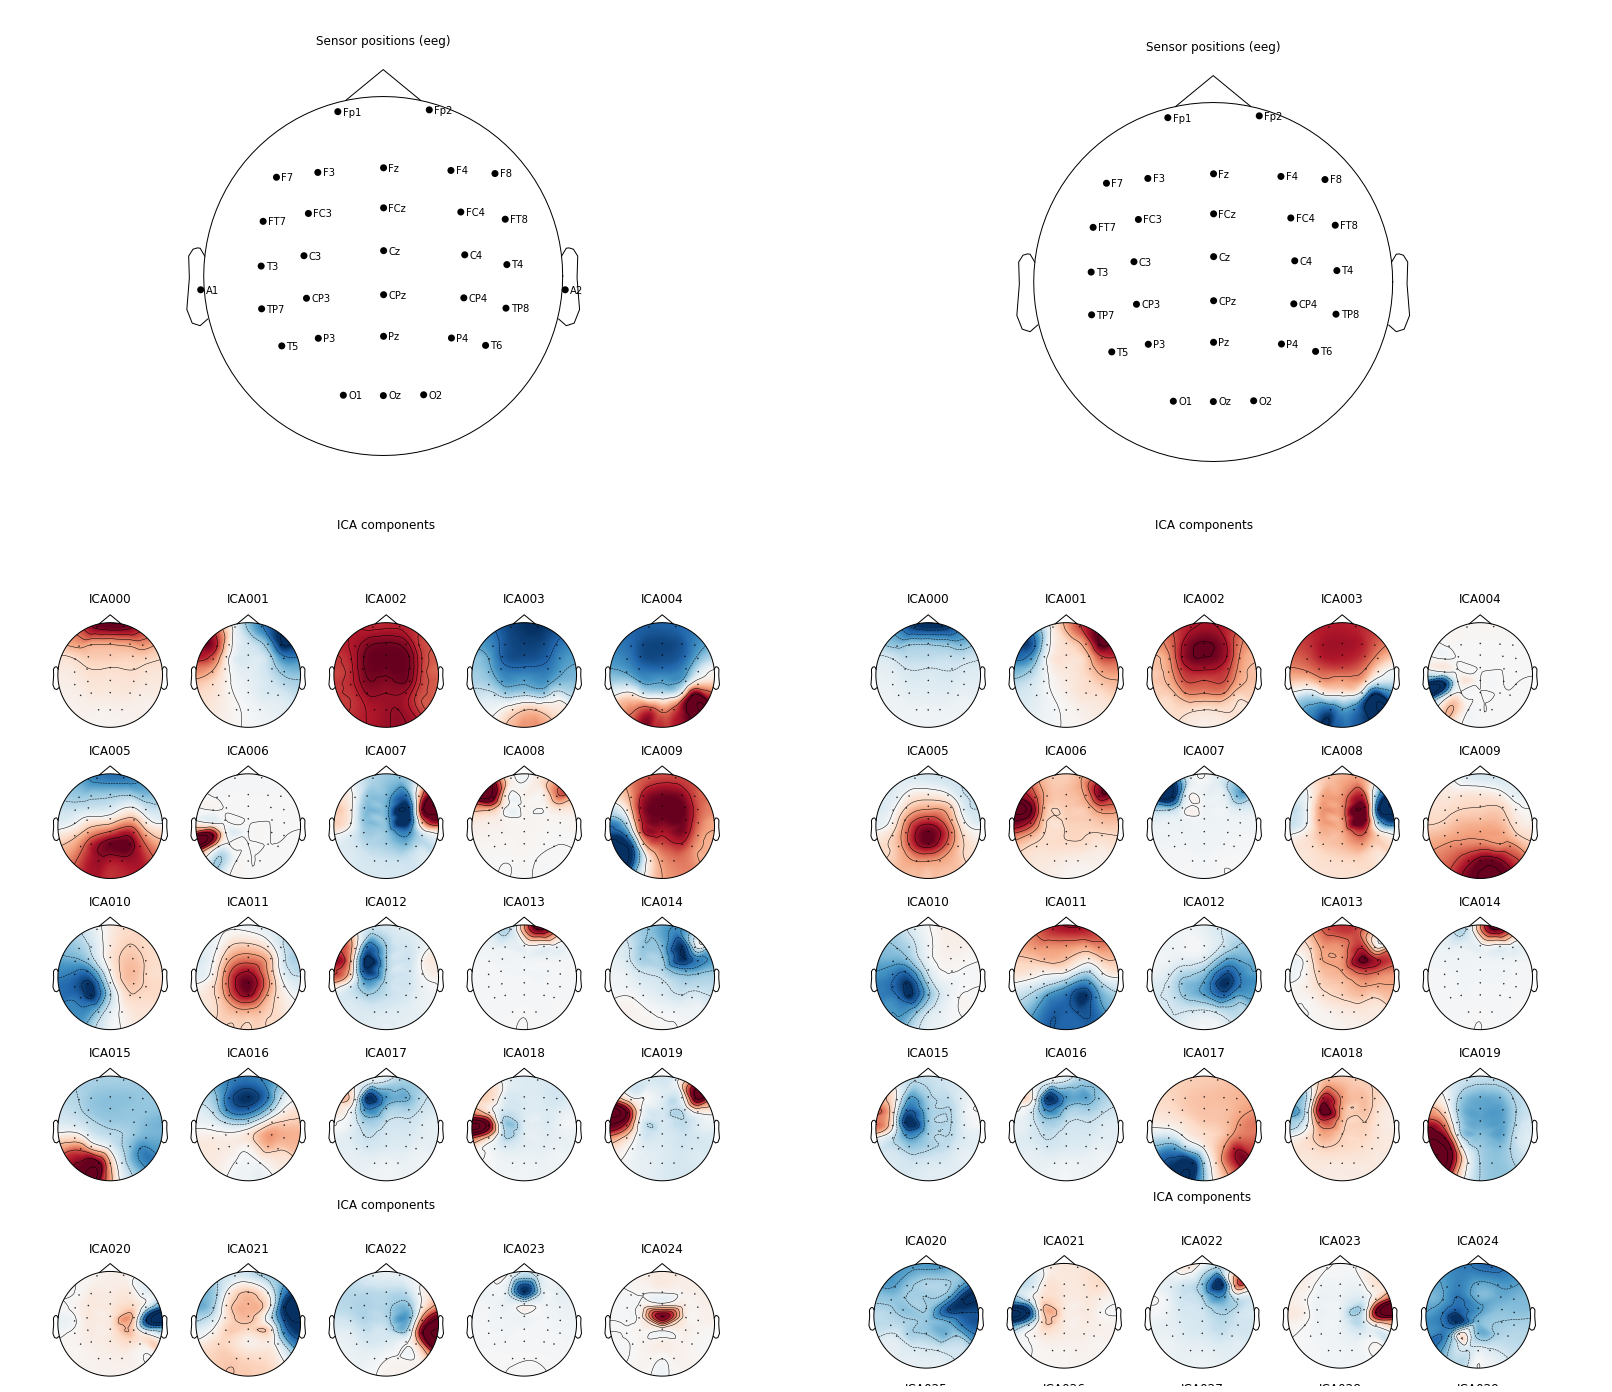
\includegraphics[height=4cm]{img/p7_8_ica.png}\\
\textcolor{red}{[b.0] (problem 7 ICA component vs problem 8 ICA component)\newline}
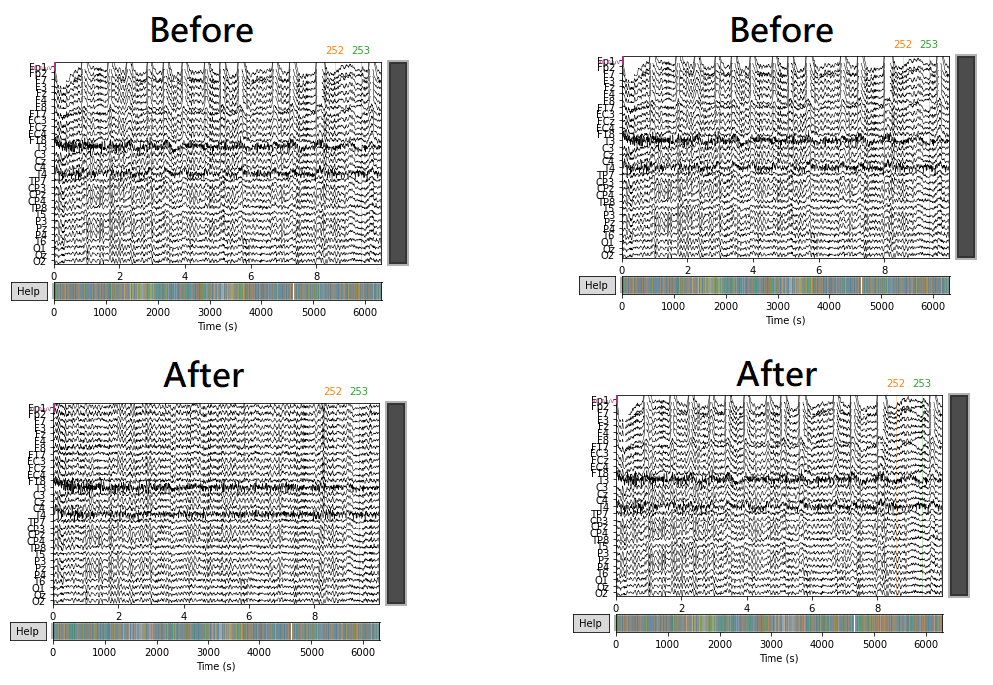
\includegraphics[height=4cm]{img/p7_8_sig.png}\\
\textcolor{red}{[b.1] (problem 7 sigmal vs problem 8 signal)\newline As we can see, both design took roughly the same time to execute, yet, the results are drastically different.  The result of the design from problem 7 is much smoother compare to the original data, but artifacts(might be muscle activities) can still be seen visually on the chart ; On the other hand, design from problem 8 does not manually identify bad components, but uses statistical approach to remove undesired components(skewness/ kurtosis/variance), the result hardly shows any differences from original data.}
\subproblem{c} Explain potential reason(s) why performance of your preprocessing strategy is superior/inferior to performance of Problem 7?
\textcolor{red}{\newline We reckoned that our design from problem 8 was inferior. Despite the fact that it is convenient to use the given function to automatically eliminate bad components, especially for unexperienced individuals, the function does not guarantee to output the optimal outcome, more often than not, it deletes the precious signal and leave the noise untouched, which is definitely NOT ideal. In our case, it deleted some of the components based on statistic factors, but the result showed little to no different from the original data, therefore retained very much the same amount of noise.}
\end{tcolorbox}
\begin{thebibliography}{6}
\bibitem{einstein} 
Kuan-Chih Huang, Chin-Teng Lin, and Tzyy-Ping Jung. \textit{Tonic and phasic eeg and behavioral changes induced by arousing feedback.} Neuroimage, 52(2):633–642, 2010.
\bibitem{Cohen} 
Mike X Cohen. \textit{Analyzing neural time series data : theory and practice.} Cambridge, Massachusetts :The MIT Press, 2014.
\bibitem{}
Chin-Teng Lin Kuan-Chih Huang and Tzyy-Ping Jung. \textit{An eeg-based fatigue detection and mitigation system.} International Journal of Neural Systems, 26(4), 2016.
%Knuth: Computers and Typesetting,
%\\\texttt{http://www-cs-faculty.stanford.edu/\~{}uno/abcde.html}
\bibitem{ICA_Naik}
Ganesh R. Naik and Dinesh K Kumar.\textit{An Overview of Independent Component Analysis and Its Applications}, Informatica, 35:63--81, 2011.
\bibitem{EEG_principal}
Donald L. Schomer and Fernando H. Lopes da Silva.
\textit{Niedermeyer's Electroencephalography: Basic Principles, Clinical Applications, and Related Fields},Lippincott William \& Wilkins, 2011. \textbf{ISBN} 9780781789424.
\bibitem{ICA_Tatsuya_Yokota}
Tatsuya Yokota. \textit{Independent Component Analysis for Blind Source Separation}, Remote Sensing, 3(6):1104--1138, 2012, Molecular Diversity Preservation International.
\end{thebibliography}
\newpage
\section{Feedback for Lab 2}
This part is not for grading but for understanding learning situation of each student. Please give us your feedback and comments.
\subsection{Work Division}
\begin{center}
    \begin{tabular}{||c|c|l||}
    \hline
    Student ID & Name & Be response for... ... \\\hline
    309554032 & Eric & co-designing the algorithm in problem 6, 7 and describing the result of 6, 7\\\hline
    309551176 & Jen Hsuan & co-designing the algorithm in problem 6, 7, designing the algorithm in problem 8, \\\hline
     &  & \hspace*{0.5cm}describing the design idea in problem 8\\\hline
    309540022 & Alexander & solving Problem 1-3 with other teammate \\\hline
    0856642 & Xu-Tao Wei &  solving Problem 1,2,4,5 with other teammate\\\hline
    0716092 & Wei-Chen Liao & solving Problem 2-3 with other teammate and discussing Problem 6-7\\\hline
    0716085 & Pin-Hua Lai & solving Problem 1-5 with other teammate, edit latex file, \\\hline
     &  & \hspace*{0.5cm}and participating discussion of Problem 6-8\\\hline
\end{tabular}
\end{center}
\subsection{Suggestions and Comments}
\subsubsection{For instructor}
\subsubsection{For teaching assistant(s)}
\textcolor{red}{1. Giving example code would be significantly helpful to this assignment.\newline 2. If some math formulas or equations can be explained more or add more friendly references would be better, especially for students without that much knowledge in some fields like signal processing, etc.\newline
}
\textbf{4.2.2.a For Min-Jiun}\\
\textbf{4.2.2.b For Eric}\\
\noindent{\color{LightRubineRed} \rule{\linewidth}{0.5mm}}
\begin{center}
    \large{\textbf{Office Hour Information}}
\end{center}
\par We'll have limited time to teach EEGLab and MNE on our course; therefore, if you have any question about lab 2, feel free to make an appointment or come to ask me during my office hour.\\
\begin{center}
    \begin{tabular}{||c|c|c||}
    \hline
    Day & Time & Office\\
        \hline\hline
          Tue. & 12:20 p.m.-13:10 p.m. & EC120 \\
          \hline
          Thur. & 06:30 p.m.-09:30 p.m. & SC207\\
          \hline
    \end{tabular}
\end{center}
\textbf{Note}\\
Actually, my office hour on Thursdays is main for calculus consultation. If there are undergraduate students come to ask calculus problems, I need to teach them first and then to solve your problem during the rest of the office hour on Thursday nights.\\
\noindent{\color{LightRubineRed} \rule{\linewidth}{0.5mm}}
\end{document} 
